\documentclass{beamer}

\mode<presentation>
%\mode<handout>
{
  \usetheme{Luebeck}
  \usecolortheme{beaver}
  % or ...

  \setbeamercovered{transparent}
  % or whatever (possibly just delete it)
}

\usepackage[english]{babel}
% \usepackage[latin1]{inputenc}
\usepackage{times}
% \usepackage[T1]{fontenc}
% \usepackage{natbib}
% \usepackage[natbib=true, bibstyle=authoryear, citestyle=authoryear-comp]{biblatex}
\usepackage{multirow}
\usepackage{rotating}

\newcommand{\Ivec}[1]{\mbox{\boldmath $#1$}}\newcommand{\argmin}{\operatornamewithlimits{argmin}}
\newcommand{\argmax}{\operatornamewithlimits{argmax}}
\newcommand{\sgn}{\operatorname{{\mathrm sgn}}}
\newcommand{\mean}{\operatornamewithlimits{mean}}
\newcommand{\Bin}{\operatorname{{\mathrm Bin}}}
\newcommand{\Beta}{\operatorname{{\mathrm Beta}}}
\newcommand{\Gammadist}{\operatorname{{\mathrm Gamma}}}
\newcommand{\Uniform}{\operatorname{{\mathrm Uniform}}}
\definecolor{Red_c}{rgb}{1, 0, 0}
\definecolor{Grey_c}{rgb}{0.33, 0.33, 0.33}

% Or whatever. Note that the encoding and the font should match. If T1
% does not look nice, try deleting the line with the fontenc.

\title[Classification, Induction and Brain Decoding]
{Classification, Induction and Brain Decoding}

%%% \subtitle
%%% {Include Only If Paper Has a Subtitle}

\author[E.Olivetti, S.Greiner]
% {\alert{Emanuele Olivetti}\inst{1}, Susanne Greiner\inst{1}}
{Emanuele Olivetti, \alert{Susanne Greiner}}

\institute[FBK/CIMeC]
{
%  \inst{1}
  NeuroInformatics Laboratory (NILab)\\
  Bruno Kessler Foundation, Trento (FBK), Italy\\
  Center for Mind and Brain Sciences (CIMeC),
  University of Trento, Italy\\
  \url{http://nilab.fbk.eu}\\
  \url{olivetti@fbk.eu}\\
  \url{greiner@fbk.eu}}


\date[PIN2011] % (optional, should be abbreviation of conference name)
{Python in Neuroscience Workshop (EuroSciPy 2011)\\
Paris, Ecole Normale Sup\'erieure, August 29-30 2011}

\subject{}
% This is only inserted into the PDF information catalog. Can be left
% out. 



% If you have a file called "university-logo-filename.xxx", where xxx
% is a graphic format that can be processed by latex or pdflatex,
% resp., then you can add a logo as follows:

%% \pgfdeclareimage[height=1.0cm]{fbk-logo}{figs/Logo-fbk}
%% \logo{\pgfuseimage{fbk-logo}}
%% \pgfdeclareimage[height=1.0cm]{unitn-alfa-logo}{figs/Logo-unitn-alfa}
%% \logo{\pgfuseimage{unitn-alfa-logo}}


% Delete this, if you do not want the table of contents to pop up at
% the beginning of each subsection:


\AtBeginSection[]
{
  \begin{frame}<beamer>{Outline}
    \tableofcontents[currentsection,currentsubsection]
  \end{frame}
}

% \AtBeginSubsection[]
% {
%   \begin{frame}<beamer>{Outline}
%     \tableofcontents[currentsection,currentsubsection]
%   \end{frame}
% }


% If you wish to uncover everything in a step-wise fashion, uncomment
% the following command: 

% \beamerdefaultoverlayspecification{<+->}


\begin{document}

\begin{frame}
  \titlepage
\end{frame}

% \begin{frame}{Title}
%   10 minutes + question time (5 minutes).
% \end{frame}

\begin{frame}{Motivation: Brain Decoding~\cite{haynes2006decoding}}
A topic relevant for BCI and Neuroscience research...
  \begin{block}{What is \emph{brain decoding}?}
    %\begin{itemize}
    %\item The use of classification-based techniques in the field of
      %neuroimaging is known as \emph{brain decoding}. % this is from WBD2010
    %\item Brain decoding corresponds to \emph{inverse inference} where
      %stimuli are predicted from neuroimaging data. % This comes from
                                % one reviewer of the Pat.Rec. article.
    %\item \emph{Pattern discrimination}: ``can a classifier accurately
      %predict which stimulus triggered the brain 
      %data?''~\cite{pereira2008machine}
    %\end{itemize}
  \end{block}
\begin{figure}
    \centering
    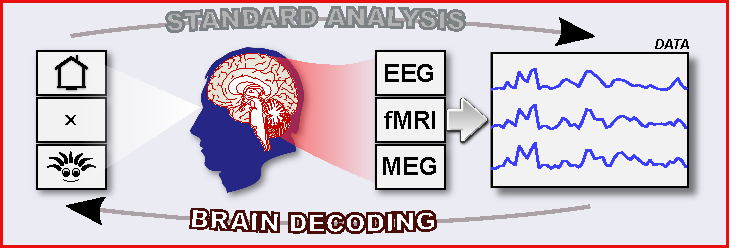
\includegraphics[width=10cm]{brain_decoding}
    \label{fig:brain_decoding}
  \end{figure}

\begin{figure}
    \centering
    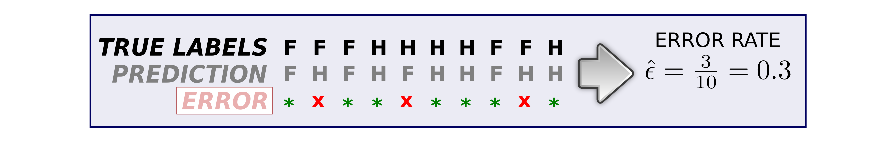
\includegraphics[width=8cm]{prediction}
    \label{fig:prediction_I}
  \end{figure}

%  \begin{block}{This is relevant to...}
%    \begin{itemize}
%    \item Brain-Computer Interface (BCI) research.
      % \begin{itemize}
      % \item Improve assistive technologies.
      % \end{itemize}
%    \item Neuroscience research, for confirmatory analysis.
      % \begin{itemize}
      % \item Confirmatory data analysis. GIVE A SHORT EXAMPLE, e.g. Knops
      %   2009? Maybe not... we are in Paris ;-).
      % \end{itemize}
%    \end{itemize}
%  \end{block}
\end{frame}

\begin{frame}{Underlying (Inductive) Questions}
  \begin{itemize}
  \item ``\emph{Is there stimulus-related information within brain
      data?}''~\cite{pereira2008machine}
  \item Information $\Longleftrightarrow$ Classification error?
  \item Is \emph{my} classifier better than the \emph{random} classifier?
  \item Did the classifier learn a thing?
  \item How to make inferences from multi-subjects experiments?
    % \item I am trying several classification algorithms (SVM, GNB,
    %   kNN, etc.) and just one works. Does this influence the
    %   evidence in favor of the presence of information?
  \end{itemize}
\begin{figure}
    \centering
    
\includegraphics[width=8cm]{prediction_II}
    \label{fig:prediction_I}
  \end{figure}

  \begin{block}{Does this really matter? YES}
    \begin{itemize}
    \item Datasets are small and very high-dimensional. It is
      difficult to have high confidence in the answers.
    % \item We believe that the literature does not (properly) answer
    %  most of those questions.
    \end{itemize}
  \end{block}
\end{frame}

\begin{frame}{Small Sample Mythology}
  \begin{itemize}
  \item The (estimated) error rate is a good performance measure.
    % When classes are unbalanced the error rate is uninformative,
    % e.g. the confusion matrix [[80, 10],[10, 0]] (predictions on
    % rows and true labels on columns) gives 20% error rate but
    % clearly the classifier did not discriminate the two classes.
    %\begin{center}
      %%% \begin{figure}
      %%%   \centering
      %%%   \includegraphics[width=10cm]{labels_ext.pdf}
      %%%   %   \label{fig:information_bayes_error_bounds}
      %%% \end{figure}
      %\begin{tabular}{ c c | r r }
        %& & \multicolumn{2}{c}{\small{\emph{true}}}\\
        %& & $\mathbf{F}$ & $\mathbf{H}$ \\
        %\hline
        %\multirow{2}{*}{\begin{sideways}\small{\emph{pred}}\end{sideways}}
        %& $\mathbf{F}$ & 90 & \alert{10} \\
        %& $\mathbf{H}$ &  0 &  0 \\
      %\end{tabular}
      %\hspace{0.5cm} $\hat{\epsilon} = \frac{10}{100} = 0.1$
    %\end{center}

\begin{columns}
    \begin{column}{5cm}
    \begin{center}
      A:
      \begin{tabular}{ c || c | c | }
            & $\mathbf{F}$ & $\mathbf{H}$ \\
        \hline
        \hline
          \textcolor{Grey_c}{$\mathbf{F}$} & 90 & \alert{10} \\
        \hline
          \textcolor{Grey_c}{$\mathbf{H}$} &  \alert{0} &  0 \\
        \hline
      \end{tabular}
      $\hat{\epsilon}=\frac{10}{100}$
    \end{center}
    \end{column}
    \begin{column}{5cm}
    \begin{center}
      B:
      \begin{tabular}{ c || c | c | }
            & $\mathbf{F}$ & $\mathbf{H}$ \\
        \hline
        \hline
          \textcolor{Grey_c}{$\mathbf{F}$} & 80 &  \alert{0} \\
        \hline
          \textcolor{Grey_c}{$\mathbf{H}$} & \alert{10} & 10 \\
        \hline
      \end{tabular}
      $\hat{\epsilon}=\frac{10}{100}$
    \end{center}
    \end{column}
  \end{columns}
\vspace{5mm}
  
columns: TRUE CLASS LABELS\\
rows: \textcolor{Grey_c}{PREDICTED CLASS LABELS}

  \item The variance of the cross-validation error rate.
    (\url{http://hunch.net/?p=29}) \cite{bengio2004no}
    % The variance of the cross-validation error rate estimate is
    % the population variance of the observed error rates across
    % folds.
    %%%%%%  \item The permutation test is reliable. (????)
    % There is no clear reference for this myth so we might end up
    % removing the item. But I've an example in mind...
  \item The error rate is Gaussian distributed.
  \item When doing multi-subject inferences the within-subject
    variance can be neglected.
  \end{itemize}
% Note: the last paper Carlton (Neuroimage 2011) is based on a dataset
% of 18 examples...
\end{frame}


\begin{frame}{Our Answers}
  \begin{enumerate}
  \item Information $\Longleftrightarrow$ Classification error?\\
    \cite{olivetti2011testing}
  \item Did the classifier learn a thing? \\ 
    $[$Current Work$]$
  \item How to make inferences from multi-subjects experiments? \\
    \cite{olivetti2011bayesian}
  \end{enumerate}
\end{frame}


\begin{frame}{1. Information $\Leftrightarrow$ good classif.?~\cite{olivetti2011testing}}
    % \begin{equation}
    %   \label{eq:bayes_error_bounds}
    %   h^{-1}(1-I(X;Y)) \leq \epsilon_B \leq \frac{1-I(X;Y)}{2}
    % \end{equation}    
  \begin{figure}
    \centering
    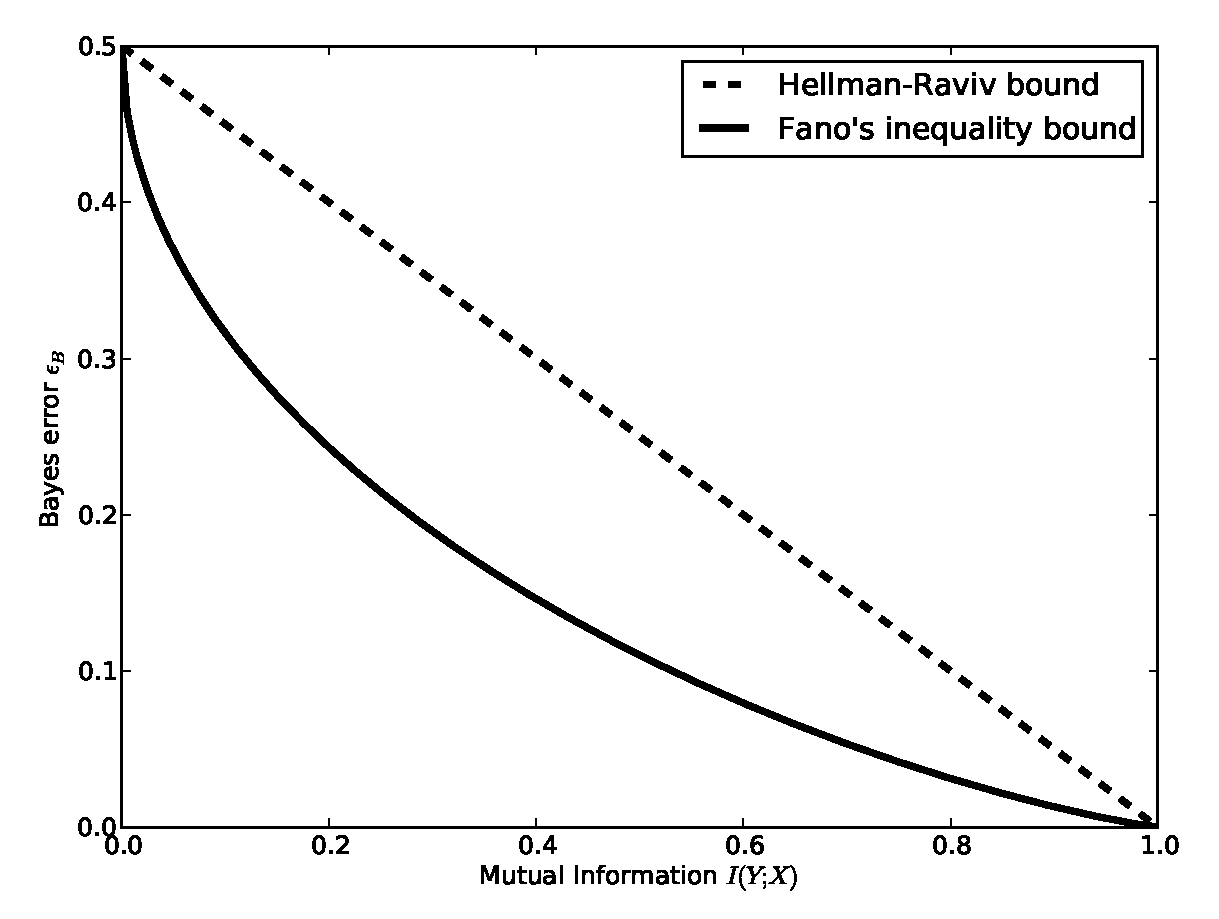
\includegraphics[width=8.5cm]{mi_be_bounds}
    \caption{Plot of the Fano's and Hellman-Raviv's inequalities in
      terms of mutual information and Bayes error \emph{for the binary
        balanced case}.}
    \label{fig:information_bayes_error_bounds}
  \end{figure}
  % \item Show Fano's and Hellman-Raviv's bounds.
  % \item Show the proposed hierarchical model
  % \item Show posterior distribution of information.
\end{frame}


\begin{frame}{2. Did the classifier learn a thing? $[$Current Work$]$}
  \begin{itemize}
  \item All tests in the literature are based on the \emph{error
      rate}.
  \item Is the error rate an appropriate measure? Examples:

\begin{columns}
    \begin{column}{5cm}
    \begin{center}
      A:
      \begin{tabular}{ c || c | c | }
            & $\mathbf{F}$ & $\mathbf{H}$ \\
        \hline
        \hline
          \textcolor{Grey_c}{$\mathbf{F}$} & 90 & \alert{10} \\
        \hline
          \textcolor{Grey_c}{$\mathbf{H}$} &  \alert{0} &  0 \\
        \hline
      \end{tabular}
      $\hat{\epsilon}=\frac{10}{100}$
    \end{center}
    \end{column}
    \begin{column}{5cm}
    \begin{center}
      B:
      \begin{tabular}{ c || c | c | }
            & $\mathbf{F}$ & $\mathbf{H}$ \\
        \hline
        \hline
          \textcolor{Grey_c}{$\mathbf{F}$} & 80 &  \alert{0} \\
        \hline
          \textcolor{Grey_c}{$\mathbf{H}$} & \alert{10} & 10 \\
        \hline
      \end{tabular}
      $\hat{\epsilon}=\frac{10}{100}$
    \end{center}
    \end{column}
  \end{columns}



\item Our approach: test of independence of predicted vs. true
  class-labels.% Let's not disclose the work of Casella now
               % ~\cite{casella2009assessing}
    \begin{itemize}
    \item A: $p(\text{independent}|\text{data}) = 76\%$
    \item B: $p(\text{independent}|\text{data}) = 0.00015\%$
    \end{itemize}
  \end{itemize}
  \begin{block}{Claim}
    \emph{accurate inference from small samples requires
      something more than the error rate, even when classes are not
      strongly unbalanced.}
  \end{block}
\end{frame}


\begin{frame}{3. Inductive reasoning about the population}
  \begin{center}
    ``\emph{Is there information at the population level?}''
  \end{center}
  
  \begin{columns}[t]
    \begin{column}{5.5cm}
      \begin{block}{Standard Procedure}
        \begin{enumerate}
        \item The error rate Gaussian.
        \item No \emph{within-}subject variance.
        \item $t$-test.
        \item Classical hyp. testing.
        \item $p\text{-value} \leq 0.05$ $\Rightarrow$ inform.
        \end{enumerate}
      \end{block}
    \end{column}
    \begin{column}{5.5cm}
      \begin{block}{\cite{olivetti2011bayesian}}
        \begin{enumerate}
        \item No Gauss. approx. $\rightarrow$ Beta.
        \item Account for $\hat{\epsilon}_i$ uncertainty.
        \item Hierarchical model.
        \item Bayesian hyp. testing.
        \item Bayes factor $\geq 3$ $\Rightarrow$ inform.
        \end{enumerate}
      \end{block}
    \end{column}
  \end{columns}
\end{frame}


\begin{frame}{Python, NumPy, SciPy...}
  \begin{itemize}
  \item Broadcasting/Vectorize magic in NumPy: ``Broadcasting provides
    a means of vectorizing array operations so that looping occurs in
    C instead of
    Python.''%\url{http://docs.scipy.org/doc/numpy/user/basics.broadcasting.html}
  \item Sampling from a hierarchical model~\cite{olivetti2011bayesian}:\\
  ``\emph{15 subjects, test set of size 50, 100k iterations: \alert{1.67 sec.}}''\\
  See \texttt{cool\_broadcasting\_vectorize.py}\\
  \item Implementation of our algorithms is freely available:\\
    %\url{https://github.com/emanuele}.
    \small{\url{github.com/emanuele/information_test}}\\
    \small{\url{github.com/emanuele/Bayes-factor-multi-subject}}\\
    ...
  \item Of course we are big fans (and sometimes contributors) of
    PyMVPA, scikits.learn, PyMC, NiPy (Dipy, nibabel,...)!
  \item We hope to send pull requests soon :-)
  \end{itemize}
\end{frame}

\begin{frame}
  \begin{center}
    \LARGE{\alert{Thank You!}}
  \end{center}
  \begin{center}
    slides available at:
    \url{https://github.com/emanuele/pin2011}
  \end{center}
\end{frame}

\begin{frame}{Inductive reasoning about population}
  ``\emph{Is there information at the population level?}''
  \begin{block}{Ex.: predict mental calculation from PSPL
      ~\cite{knops2009recruitment}}
    \begin{itemize}
    \item test set size: $108$ presentations $\times$ $15$ subjects.
    \item $\{ 43, 59, 51, 38, 39,  53, 47, 50, 50, 59, 59, 45, 36, 46,
      53 \}$.
    \end{itemize}
  \end{block}
  \begin{columns}[T]
    \begin{column}{5.5cm}
      \begin{block}{$t$-test}
        \begin{figure}
          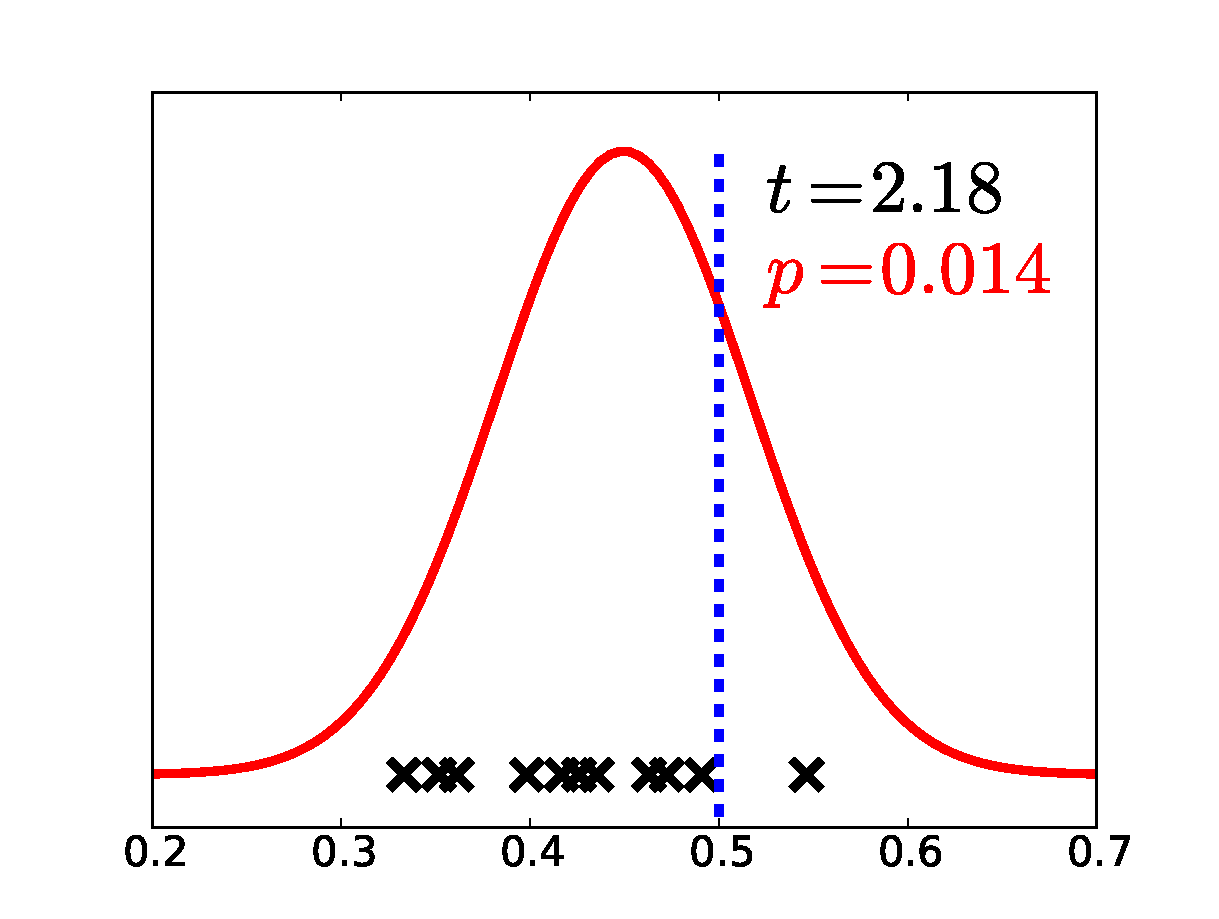
\includegraphics[width=4.5cm]{knops}
        \end{figure}
        %$t=2.18$, $\alert{p=0.014}$
      \end{block}
    \end{column}
    \begin{column}{5.5cm}
      \begin{block}{\cite{olivetti2011bayesian}}
        \begin{itemize}
        \item No Gauss. approx. $\rightarrow$ Beta.
        \item Account for $\hat{\epsilon}_i$ uncertainty.
        \item Hierarchical model.
        \item Bayesian hyp. testing.
        \item \alert{$B_{\text{Inf}/\text{NoInf}}=2.5$} (weak)
        \end{itemize}
      \end{block}
    \end{column}
  \end{columns}
\end{frame}


\bibliographystyle{apalike}
% \bibliographystyle{plainnat}  

\bibliography{emanueleolivetti-pin2011}


\end{document}
